% Diagrama conceptual de la estructura de un modelo oculto de Markov (capítulo 2,
% §2.3). Cadena de estados ocultos S_t (transición A) que emiten observaciones O_t.
% Ilustrativo (no es figura de decisión). Compila standalone a PDF y se incluye con
% 
\includegraphics{figuras/prelim_hmm.pdf}.
\documentclass[border=8pt]{standalone}
\usepackage[T1]{fontenc}
\usepackage[utf8]{inputenc}
\usepackage{lmodern}
\usepackage{amsmath}
\usepackage{tikz}
\usepackage{xcolor}
\usetikzlibrary{arrows.meta, positioning}

\definecolor{azul}{HTML}{1F4E79}
\definecolor{azulclaro}{HTML}{DAE8F5}
\definecolor{gris}{HTML}{555555}
\definecolor{grisclaro}{HTML}{ECECEC}

\begin{document}
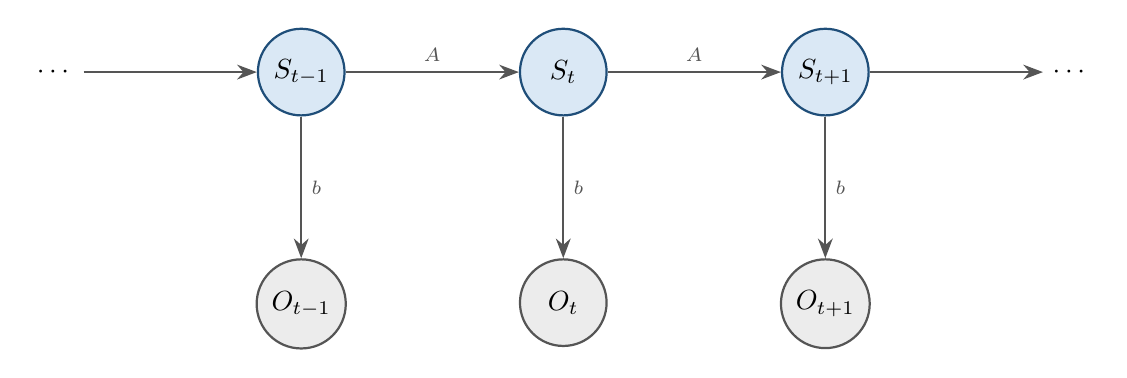
\begin{tikzpicture}[
  font=\sffamily,
  oculto/.style={circle, draw=azul, thick, fill=azulclaro, minimum size=1.1cm},
  obs/.style={circle, draw=gris, thick, fill=grisclaro, minimum size=1.1cm},
  arr/.style={-{Stealth[length=2.5mm]}, thick, gris},
  lbl/.style={font=\sffamily\scriptsize\itshape, text=gris},
  node distance=2.2cm,
]

% --- Cadena oculta (fila superior) ---
\node (sa) {$\cdots$};
\node[oculto, right=of sa] (s1) {$S_{t-1}$};
\node[oculto, right=of s1] (s2) {$S_{t}$};
\node[oculto, right=of s2] (s3) {$S_{t+1}$};
\node[right=of s3] (sb) {$\cdots$};

% --- Observaciones (fila inferior) ---
\node[obs, below=1.8cm of s1] (o1) {$O_{t-1}$};
\node[obs, below=1.8cm of s2] (o2) {$O_{t}$};
\node[obs, below=1.8cm of s3] (o3) {$O_{t+1}$};

% --- Transiciones de la cadena oculta ---
\draw[arr] (sa) -- (s1);
\draw[arr] (s1) -- node[lbl, above]{$A$} (s2);
\draw[arr] (s2) -- node[lbl, above]{$A$} (s3);
\draw[arr] (s3) -- (sb);

% --- Emisiones ---
\draw[arr] (s1) -- node[lbl, right]{$b$} (o1);
\draw[arr] (s2) -- node[lbl, right]{$b$} (o2);
\draw[arr] (s3) -- node[lbl, right]{$b$} (o3);

\end{tikzpicture}
\end{document}
